\documentclass[twocolumn]{rbef}

\usepackage{lipsum}

\usepackage{bbm}
\usepackage{subfig}
\usepackage{pdfpages} % Para incluir a capa.

\hypersetup{%
    pdfborder = {0 0 0}
}

\newcommand{\1}{\mathbbm{1}}
\newcommand{\s}{\mathcal{S}}
\newcommand{\T}{\mathcal{T}}
\newcommand{\A}{\mathcal{A}}
\newcommand{\ket}{\rangle}
\newcommand{\bra}{\langle}

\newcommand*{\secref}[1]{\ref{#1}}

\newtheorem{defi}{Definição}
\newtheorem{theorem}{Teorema}
\newtheorem{acknowledgement}[theorem]{Acknowledgement}
\newtheorem{algorithm}[theorem]{Algorithm}
\newtheorem{axiom}[theorem]{Axiom}
\newtheorem{claim}[theorem]{Claim}
\newtheorem{conclusion}[theorem]{Conclusion}
\newtheorem{condition}[theorem]{Condition}
\newtheorem{conjecture}[theorem]{Conjecture}
\newtheorem{corollary}[theorem]{Corollary}
\newtheorem{criterion}[theorem]{Criterion}
\newtheorem{definition}[theorem]{Definition}
\newtheorem{example}[theorem]{Example}
\newtheorem{exercise}[theorem]{Exercise}
\newtheorem{lemma}[theorem]{Lemma}
\newtheorem{notation}[theorem]{Notation}
\newtheorem{problem}[theorem]{Problem}
\newtheorem{proposition}[theorem]{Proposition}
\newtheorem{remark}[theorem]{Remark}
\newtheorem{solution}[theorem]{Solution}
\newtheorem{summary}[theorem]{Summary}
\newenvironment{proof}[1][Proof]{\noindent\textbf{#1.} }{\ \rule{0.5em}{0.5em}}

\titulocabecalho{Classificação de Churn Utilizando um Modelo de Regressão Logística}
\autorcabecalho{Antonio C. da Silva Júnior}

\numeracao{01}
\volume{01}
\numero{01}
\ano{2019}
\doi{http://dsbd.leg.ufpr.br/tcc}
% \tipodeartigo{TCC DSBD}
\tipodeartigo{Especialização em Data Science \& Big Data}
% \addtocounter{page}{566} %% \setcounter produces extra white page!!! use ===\addtocounter===

\author[]{Antonio C. da Silva Júnior}

\affil[]{Campus Santos, Universidade Paulista, Av. Conselheiro Nébias 766, Boqueirão, 11045-002, Santos, SP, Brasil\thanks{\href{emailto:juniorssz@gmail.com}{\href{mailto:juniorssz@gmail.com}{\nolinkurl{juniorssz@gmail.com}}}}
}
\titulo{Classificação de Churn Utilizando um Modelo de Regressão Logística}

\subtitulo{Customer Churn Classification Using a Logistic Regression Model}

% -----------------------------------------------------------------------

\begin{document}

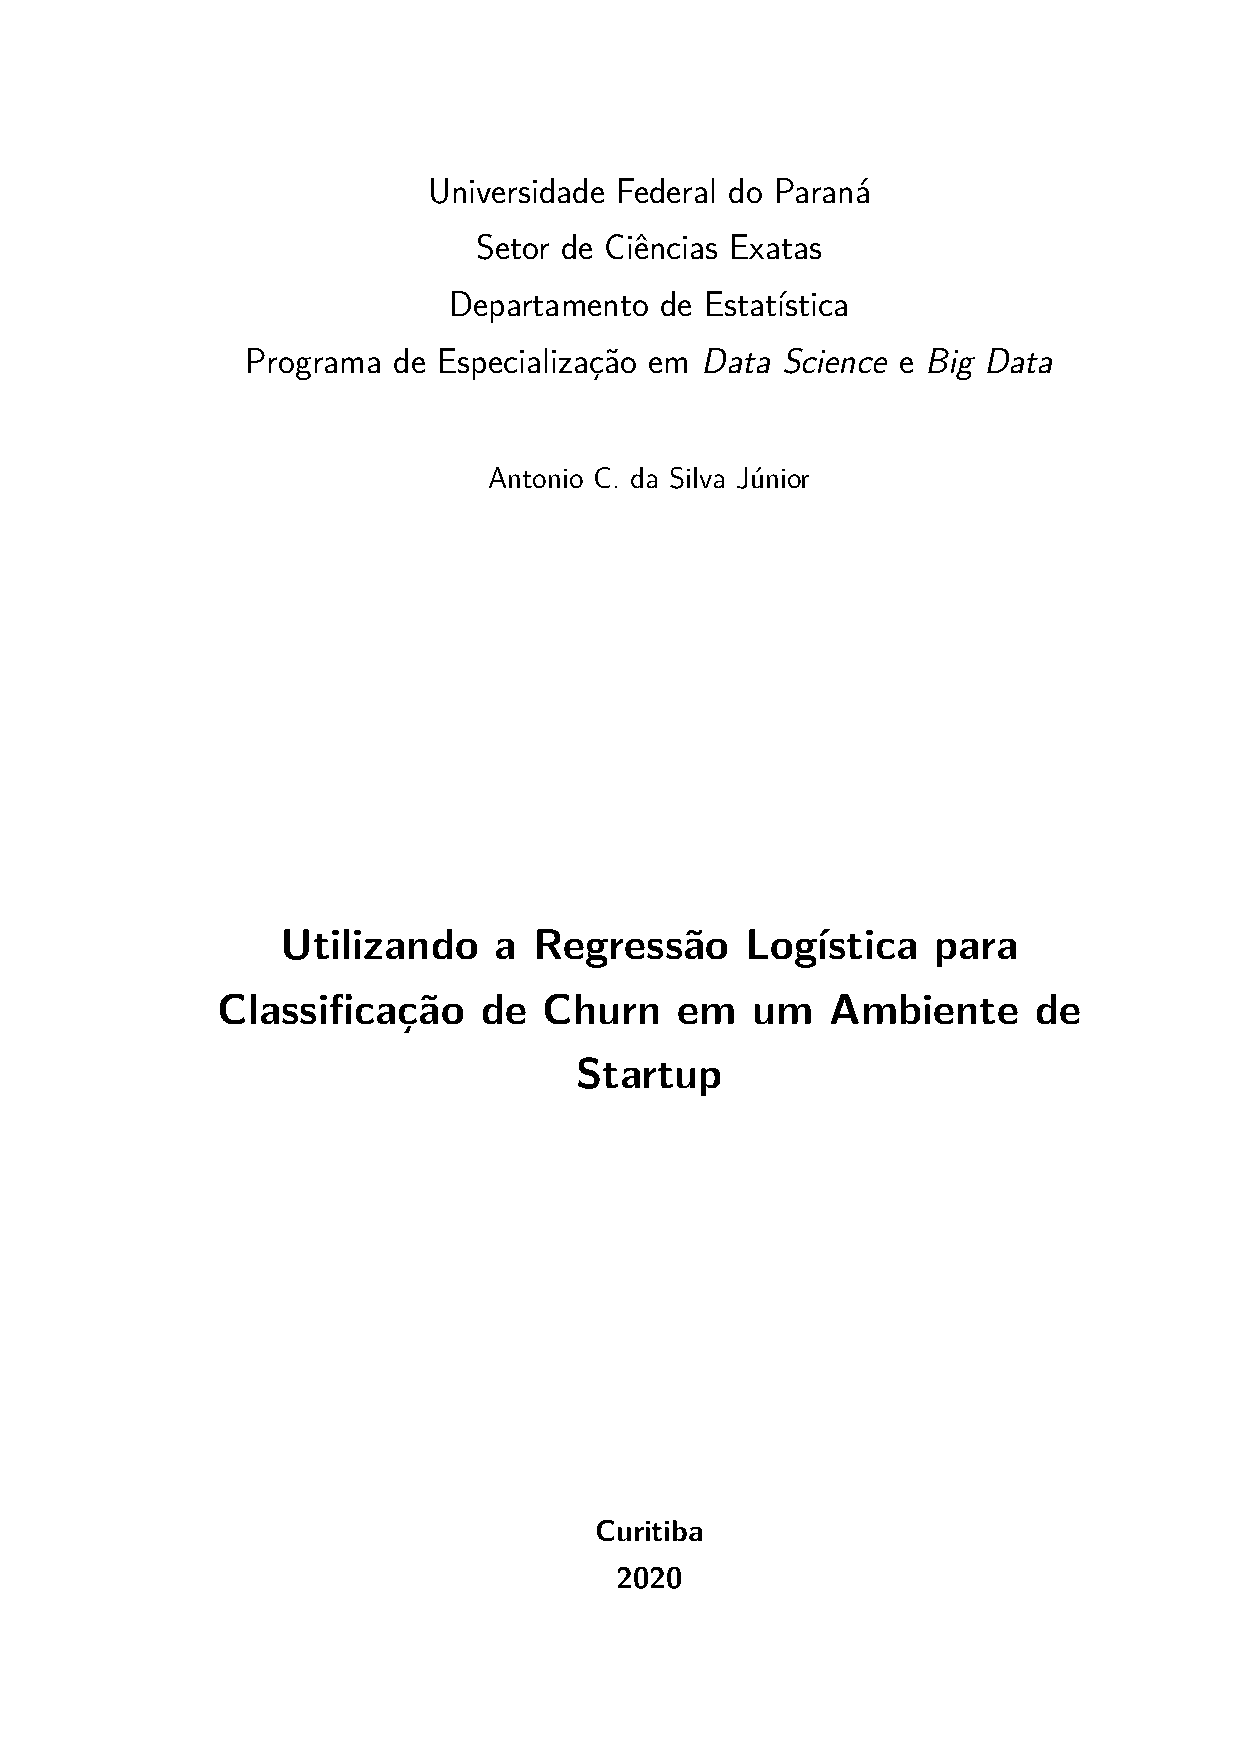
\includepdf[pages=-]{cover.pdf} % Incluí a capa

\begin{primeirapagina}

  % \begin{center}
  %   \vspace{-12pt} \small{Recebido em xxx. Aceito em xxx}
  % \end{center}

  \begin{abstract}
    O desenvolvimento de estratégias para retenção de clientes se tornou uma prática comum entre companhias de diversos segmentos, uma vez que relacionamentos de longo prazo com clientes estão associados à sobrevivência econômica e ao sucesso das empresas. Portanto, com o objetivo de antever clientes propensos a abandonar o relacionamento com uma startup brasileira, fenômeno conhecido como \textit{churn}, este artigo apresenta um modelo preditivo que possibilita a classificação de \textit{churn} e permite a interpretação dos motivos que impactam o desfecho. Após um extensivo processo de \textit{data wrangling}, aplicou-se a regressão logística fazendo uso de validação cruzada K-fold e do algortimo \textit{stepwise} para seleção de covariáveis. O modelo final, composto por 14 covariáveis, passou por uma análise de diagnóstico por meio dos resíduos quantilicos aleatorizados e teve o poder preditivo avaliado através da curva ROC, matriz de confusão e de métricas de avaliação. Em todas as etapas do estudo o modelo foi considerado adequado para o negócio e, além de exibir um bom poder preditivo, demonstrou-se capaz de fornecer \textit{insights} para ações de marketing personalizadas e otimizadas com foco na retenção dos clientes propensos a dar \textit{churn}.
    \palavraschave{Churn, Retenção de clientes, CRM, Regressão logística, Stepwise.}

  \end{abstract}

  \begin{otherlanguage}{english}

    \begin{abstract}
      Developing strategies for customer retention became a common practice among companies from different segments, since long-term relationships with customers are associated to the economic survival and success of companies. Therefore, with the goal of predicting the customer churn of a Brazilian startup, this article presents a predictive model that classifies the customer churn and allows interpreting the reasons that impact the outcome. After an extensive data wrangling process, the logistic regression was applied using K-fold cross-validation and the stepwise algorithm for covariate selection. The final model, composed by 14 covariates, has undergone a diagnostic analysis through randomized quantile residuals and its prediction power was evaluated by the ROC curve, confusion matrix and evaluating metrics. The model was considered appropriate for the business in all stages of the study and not only proved to have a good prediction power, but also demonstrated to be capable of providing insights for executing optimized and customized marketing actions focusing on the retention of customers likely to churn.
      \keywords{Customer churn, Customer retention, CRM, Logistic regression, Stepwise}

    \end{abstract}
  \end{otherlanguage}

\end{primeirapagina}
\saythanks

\hypertarget{introduuxe7uxe3o}{%
\section{Introdução}\label{introduuxe7uxe3o}}

A importância do relacionamento de longo prazo entre cliente e empresa é um assunto vastamente discutido na literatura. Devido aos efeitos do aprendizado e à redução dos custos de manutenção, atender um cliente se torna menos dispendioso a cada ano adicional de relacionamento \cite{Ganesh2000}. Por conta do aumento dos custos para atração de novos clientes em um mercado competitivo e a potencial redução dos custos associados aos relacionamentos de longo prazo, a retenção de clientes se torna essencial para a sobrevivência econômica e o sucesso das empresas do setor de serviços \cite{HennigThurau2004}. De acordo com Gallo \cite{Gallo2014}, dependendo do estudo e do segmento no qual a empresa está inserida, o custo para adquirir um novo cliente pode ser de cinco a vinte e cinco vezes superior ao da manutenção de um cliente já existente.

O desenvolvimento de estratégias para retenção de clientes se tornou uma prática comum entre companhias de diversos segmentos, e em consequência, antever os clientes propensos a abandonar o relacionamento com a empresa, fenômeno conhecido como \textit{churn}, se tornou um anseio constante. Em um momento de generalizados esforços na direção da cultura orientada a dados, os modelos preditivos para detecção de \textit{churn}, predominantemente utilizados por grandes companhias no setor de telecomunicações, se tornaram ferramentas populares nas empresas, independentemente da magnitude e da área de atuação.

A literatura comprova que a modelagem preditiva para detecção de churn é um tema bastante explorado e que possibilita inúmeras maneiras de desfecho: Botelho e Tostes \cite{Botelho2010} ajustaram um modelo de regressão logística para predizer a probabilidade de \textit{churn} em uma grande empresa de varejo; Vafeiadis et al.~\cite{Vafeiadis2015} tiveram sucesso, entre os métodos comparados, na classificação de churn através do SVM (kernel polinomial) com AdaBoost em uma empresa de telecomunicações; Baseados nos dados de avaliações online de clientes, Kumar e Yadav \cite{Kumar2020} propuseram um modelo preditivo para detecção de churn baseado em regras, através de redes neurais artificiais e teoria dos conjuntos aproximados.

Com base nos dados disponibilizados pelo Olist, startup brasileira que tem como principal produto uma plataforma digital para conectar vendedores de diversos segmentos aos grandes marketplaces, a proposta deste artigo é apresentar um modelo preditivo que possibilite não só a classificação de vendedores propensos a abandonar o relacionamento com a empresa, mas que também permita a interpretação dos motivos que possivelmente estejam impactando o desfecho. Diante da variedade de técnicas disponíveis e das particularidades de cada modelo de negócio, a escolha do algoritmo adequado se torna uma etapa crucial do processo de modelagem. Portanto, tendo como referência a abordagem de Silva Júnior, Almeida e Santos \cite{Junior2020}, que utilizaram uma modelagem híbrida multicritério considerando múltiplos decisores para a escolha de um modelo preditivo de \textit{churn}, o algoritmo escolhido para desenvolver o classificador proposto foi a regressão logística.

\hypertarget{materiais-e-muxe9todos}{%
\section{Materiais e métodos}\label{materiais-e-muxe9todos}}

\hypertarget{estruturauxe7uxe3o-do-conjunto-de-dados}{%
\subsection{Estruturação do conjunto de dados}\label{estruturauxe7uxe3o-do-conjunto-de-dados}}

Os dados utilizados neste trabalho referem-se a clientes do Olist e foram disponibilizados anonimizados e com variáveis quantitativas padronizadas com média 0 e desvio padrão 1. Considerando que estes clientes contrataram uma plataforma digital que possibilita a venda de produtos nos principais marketplaces, neste trabalho eles serão chamados de vendedores. Devido às características da arquitetura do banco de dados e às particularidades do negócio da companhia, houve a necessidade de realizar um longo processo de \textit{data wrangling}. Este processo inicia-se por um diagnóstico preliminar dos dados, ou seja, se estão no formato adequado, se respondem as perguntas que motivaram a análise e o que é necessário para colocá-los no formato ideal. Em seguida avalia-se a ocorrência de dados faltantes, valores inconsistentes e duplicatas e, por fim, realiza-se um processo de limpeza e transformação, de modo a se obter um conjunto de dados adequado para o estudo \cite{Kandel2011}.

\hypertarget{definiuxe7uxe3o-da-variuxe1vel-resposta-e-covariuxe1veis-de-desempenho}{%
\subsubsection{Definição da variável resposta e covariáveis de desempenho}\label{definiuxe7uxe3o-da-variuxe1vel-resposta-e-covariuxe1veis-de-desempenho}}

Inicialmente foram definidos como \textit{churn} (\(Y=1\)) os vendedores que estiveram inativos por 30 dias corridos desde a data da última atividade e permaneceram no mesmo estado em definitivo, considerando como atividade o acesso à plataforma digital ou a ocorrência de uma venda online. Em seguida, em função da data de corte estabelecida conforme a Tabela \ref{tab:dataDeCorte}, foram mantidos no conjunto de dados somente os vendedores com pelo menos 90 dias de histórico. O período de 90 dias, finalizado na data de corte, foi dividido igualmente em dois subperíodos, onde foram calculadas métricas como faturamento, ticket médio, quantidade de produtos publicados, quantidade de pedidos cancelados, número de dias em atividade e etc., em cada cada um dos subperíodos. Em seguida, através da equação \(V2 / (V1 + V2)\), foi calculado o desempenho do vendedor em função de diversas métricas, sendo \(V1\) e \(V2\) os valores calculados para cada subperíodo.

As métricas desempenho, dada a natureza da equação de origem, possuem o comportamento explicado pela Tabela \ref{tab:metricas}. Ao término desta etapa foi obtido um conjunto de dados composto pela variável resposta (\textit{churn}) e, como covariáveis, 9 métricas de desempenho, onde cada observação representa um vendedor.

\begin{table}

\caption{\label{tab:dataDeCorte}Definição da data de corte}
\centering
\fontsize{9}{11}\selectfont
\begin{tabular}[t]{ll}
\toprule
Vendedor & Data de corte\\
\midrule
Definido como churn & Última atividade\\
Em atividade normal & Realização da análise\\
\bottomrule
\end{tabular}
\end{table}

\begin{table}

\caption{\label{tab:metricas}Interpretação das métricas de desempenho}
\centering
\fontsize{9}{11}\selectfont
\begin{tabular}[t]{ll}
\toprule
Valor & Desempenho\\
\midrule
0,5 & Mantido\\
> 0,5 & Aumentado\\
< 0,5 & Reduzido\\
\bottomrule
\end{tabular}
\end{table}

\hypertarget{adiuxe7uxe3o-de-outras-covariuxe1veis}{%
\subsubsection{Adição de outras covariáveis}\label{adiuxe7uxe3o-de-outras-covariuxe1veis}}

Foram adicionadas covariáveis qualitativas que representam o estágio do vendedor, o plano contratado e a região de origem, bem como covariáveis quantitativas como o faturamento total, total de produtos publicados, quantidade total de pedidos e etc., resultando em um conjunto de dados com 23 covariáveis.

\hypertarget{criauxe7uxe3o-de-covariuxe1veis-binuxe1rias}{%
\subsubsection{Criação de covariáveis binárias}\label{criauxe7uxe3o-de-covariuxe1veis-binuxe1rias}}

Dada a necessidade de analisar o comportamento da variável resposta em função de uma covariável qualitativa com \(n\) categorias, deve-se criar \(n-1\) covariáveis binárias (dummies), que assumem valores iguais a 0 ou 1, ficando por conta do pesquisador decidir qual das categorias será a referência (dummy = 0) \cite{Favero2017}. Portanto, as covariáveis qualitativas adicionadas foram transformadas em binárias, resultando em um conjunto de dados composto por 32 variáveis e 11.131 observações.

\hypertarget{modelo-de-regressuxe3o-loguxedstica}{%
\subsection{Modelo de regressão logística}\label{modelo-de-regressuxe3o-loguxedstica}}

O objetivo da regressão logística é o estudo da probabilidade de ocorrência de um evento de interesse (\(Y\)), apresentado na forma dicotômica (\(Y=1\) se o evento de interesse ocorrer; \(Y=0\), caso contrário), em função de um vetor de covariáveis (\(X_1, ..., X_n\)). Sua definição ocorre através da Equação \eqref{eq:logito}, onde \(\beta_j\) (\(j = 0,1,2,...,p\)) representa os parâmetros a serem estimados, sendo \(\beta_0\) o intercepto e os demais, parâmetros de cada covariável. E o subscrito \(i\) representa cada observação da amostra (\(i = 1, 2,...,n\)) \cite{Favero2017}.
\begin{equation}
\ln \left ( \dfrac{\pi_i}{1-\pi_i} \right ) = \beta_0 + \beta_1 X_{i1} + ... +  \beta_p X_{ip}\label{eq:logito}
\end{equation}

A Equação \eqref{eq:logito} modela a log-chance de ocorrência do evento de interesse, portanto, para obter uma expressão para a probabilidade de ocorrência do evento é necessário isolar matematicamente \(\pi_i\), resultando na Equação \eqref{eq:probabilidade}.
\begin{equation}
\pi_i = \dfrac{1}{1 + e^{-(\beta_0 + \beta_1 X_{i1} + ... +  \beta_p X_{ip})}}\label{eq:probabilidade}
\end{equation}

A estimação dos parâmetros \(\beta_j\) é realizada por máxima verossimilhança, método que consiste em encontrar os parâmetros que maximizam a função de verossimilhança representada através da Equação \eqref{eq:verossimilhanca}.
\begin{equation}
L =  \prod_{i=1}^{n} \left[ \pi_i^{Y_i} (1-\pi_i)^{1-Y_i} \right]\label{eq:verossimilhanca}
\end{equation}

Entretanto, matematicamente é mais conveniente trabalhar com o logaritmo da função de verossimilhança, conhecido como função de log-verossimilhança \cite{Favero2017,Botelho2010}, representado através da Equação \eqref{eq:logverossimilhanca}.

\begin{equation}
\log L = \sum_{i=1}^{n} \left\{ \big[Y_i\ln(\pi_i)\big] + \big[(1-Y_i)\ln(1-\pi_i)\big] \right\}\label{eq:logverossimilhanca}
\end{equation}

\hypertarget{ajuste-do-modelo-e-seleuxe7uxe3o-de-covariuxe1veis}{%
\subsection{Ajuste do modelo e seleção de covariáveis}\label{ajuste-do-modelo-e-seleuxe7uxe3o-de-covariuxe1veis}}

A comparação entre dois modelos de regressão logística pode ser realizada através do Critério de Informação de Akaike (AIC), definido por \(-2\log L + 2p\), onde \(\log L\) é a log-verossimilhança maximizada e \(2p\) é o termo de penalização, sendo \(p\) o número de parâmetros do modelo, devendo-se selecionar o modelo que apresentar o menor valor de AIC. Entretanto, avaliar todas a combinações possíveis pode ser computacionalmente invivável, mesmo para um número moderado de covariáveis. Portanto, para ajudar a encontrar o melhor modelo com o menor número de covariáveis possível foi utilizado o algoritmo \textit{stepwise} \cite{Taconeli2019}. Por padrão o \textit{stepwise} utiliza a minimização do AIC como critério para seleção das covariáveis, porém, neste estudo optou-se por alterar o múltiplo de penalização do AIC de 2 para 3,841459, que corresponde ao valor do quantil da distribuição do \(\chi^2\) com 1 grau de liberdade e 5\% de significância, permitindo assim que fosse considerado o p-valor = 0,05 como valor crítico para a seleção das covariáveis em cada iteração do algoritmo.

O conjunto de dados foi separado aleatoriamente em duas partes, garantindo a proporção aproximada de 47,3\% de ocorrência de \textit{churn} (\(Y=1\)) em ambas as amostras. A amostra menor, com 25\% dos dados, foi separada para a etapa de avaliação do poder preditivo do modelo, ao passo que a amostra maior foi utilizada para o ajuste de dois modelos por valição cruzada K-fold com 5 folds \cite{Kohavi1995}, a partir de todas as covariáveis disponíveis. Um deles, denominado \textit{modelo completo}, foi ajustado da maneira tradicional, ao passo que o segundo modelo, denominado \textit{modelo restrito}, teve o ajuste realizado através do algoritmo \textit{stepwise}.

\hypertarget{resultados-e-discussuxf5es}{%
\section{Resultados e discussões}\label{resultados-e-discussuxf5es}}

\hypertarget{teste-da-razuxe3o-da-verossimilhanuxe7a}{%
\subsection{Teste da razão da verossimilhança}\label{teste-da-razuxe3o-da-verossimilhanuxe7a}}

Por meio do teste da razão da verossimilhança (TRV), representado através da Equação \eqref{eq:trv}, é possível verificar a qualidade do ajuste do \textit{modelo completo}, ajustado com \(j\) covariáveis, em comparação com o \textit{modelo restrito}, ajustado com \(j-k\) covariáveis, sendo \(k\) o número de covariáveis removidas do ajuste. Quando a estatística do TRV é inferior ao valor da distribuição do \({\chi}^2\) com \(k\) graus de liberdade e 5\% de significância, não rejeita-se a hipótese nula, ou seja, constata-se que a remoção de \(k\) covariáveis não afeta a qualidade do ajuste do modelo \cite{Favero2017}.

\begin{equation}
\text{TRV} = -2(\log L_{\text{completo}} -\log L_{\text{restrito}})\label{eq:trv}
\end{equation}

Ao realizar o teste, foi constatado que a remoção das 17 covariáveis através do algoritmo \textit{stepwise} não alterou a qualidade do ajuste, uma vez que a estatística do teste foi inferior ao valor da distribuição do \({\chi}^2\) com 17 graus de liberdade e 5\% de significância. Portanto, optou-se pelo \textit{modelo restrito} para a continuidade do estudo, uma vez que este possui complexidade inferior com relação ao \textit{modelo completo}, sem perda de qualidade. A Tabela \ref{tab:covars} exibe as 14 covariáveis selecionadas para o modelo.

\begin{table*}

\caption{\label{tab:covars}Covariáveis utilizadas pelo modelo}
\centering
\fontsize{9}{11}\selectfont
\begin{tabular}[t]{lll}
\toprule
Covariável & Descrição & Suporte\\
\midrule
\addlinespace[0.3em]
\multicolumn{3}{l}{\textbf{Métricas de desempenho}}\\
\hspace{1em}X2 & Desempenho do número de pedidos cancelados ou suspensos no período & $[0,1]$\\
\hspace{1em}X4 & Desempenho da média de dias de atraso (postagens) no período & $[0,1]$\\
\hspace{1em}X5 & Desempenho da média de dias de atraso (entregas) no período & $[0,1]$\\
\hspace{1em}X6 & Desempenho do faturamento no período & $[0,1]$\\
\hspace{1em}X9 & Desempenho do ticket médio no período & $[0,1]$\\
\addlinespace[0.3em]
\multicolumn{3}{l}{\textbf{Qualitativas}}\\
\hspace{1em}X11 & Necessita de dias adicionais para postagem & $\{0,1\}$\\
\hspace{1em}X13 & Está no estágio I & $\{0,1\}$\\
\hspace{1em}X14 & Está no estágio R & $\{0,1\}$\\
\hspace{1em}X20 & Localizado na região Sudeste & $\{0,1\}$\\
\addlinespace[0.3em]
\multicolumn{3}{l}{\textbf{Quantitativas}}\\
\hspace{1em}X22 & Valor total do faturamento & $\mathbb{R}_+$\\
\hspace{1em}X27 & Número total de produtos publicados & $\mathbb{N}$\\
\hspace{1em}X29 & Número de dias desde a contratação até a primeira venda & $\mathbb{N}$\\
\hspace{1em}X30 & Número de dias desde a contratação até estar pronto para operar & $\mathbb{N}$\\
\hspace{1em}X31 & Número de dias em atividade no período & $\mathbb{N}$\\
\bottomrule
\end{tabular}
\end{table*}

\hypertarget{anuxe1lise-de-diagnuxf3stico}{%
\subsection{Análise de diagnóstico}\label{anuxe1lise-de-diagnuxf3stico}}

Com a intenção de generalizar o método de análise dos resíduos da regressão linear para todos os modelos lineares generalizados, Dunn e Smyth \cite{Dunn1996} propuseram os resíduos quantílicos aleatorizados, definidos por \(r_i = \phi^{-1}(u_i)\), onde \(\phi^{-1}\) é a inversa da função de distribuição acumulada da normal padrão e \(u_i = F(y_i;\mu_i,\phi)\), com distribuição uniforme entre 0 e 1, é calculado com base na distribuição acumulada do modelo proposto. Caso o modelo logístico esteja bem ajustado, espera-se que os resíduos quantílicos aleatorizados se apresentem normalmente distribuídos e com variância constante \cite{Taconeli2015}. A análise da qualidade do ajuste, através dos resíduos, foi realizada de forma gráfica. Ao comparar os resíduos com os valores ajustados (Figura \ref{fig:resplot}) é possível observar que estes apresentam variabilidade aproximadamente constante e estão centrados predominantemente em 0, entre -2 e 2. No gráfico quantil-quantil \cite{Wilk1968} (Figura \ref{fig:qqplot}) nota-se que os resíduos estão, de forma razoável, aderentes à distribuição normal. Portanto, nesta etapa foi concluído que o modelo não apresentou violação dos pressupostos.

\begin{figure}

{\centering 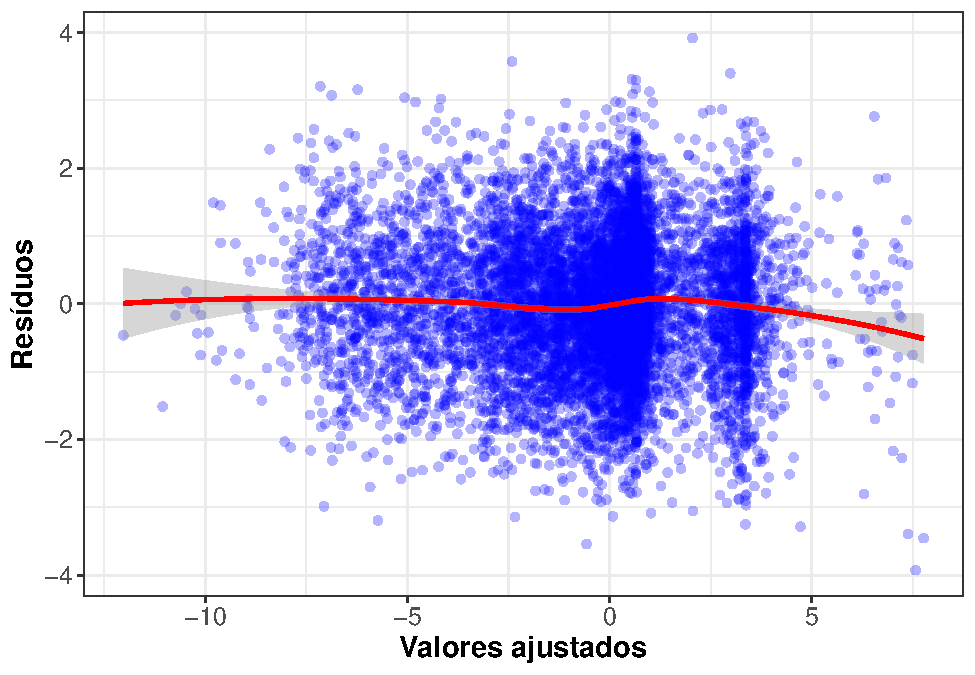
\includegraphics[width=1\linewidth]{article_files/figure-latex/resplot-1} 

}

\caption{Gráficos dos resíduos versus valores ajustados}\label{fig:resplot}
\end{figure}

\begin{figure}

{\centering 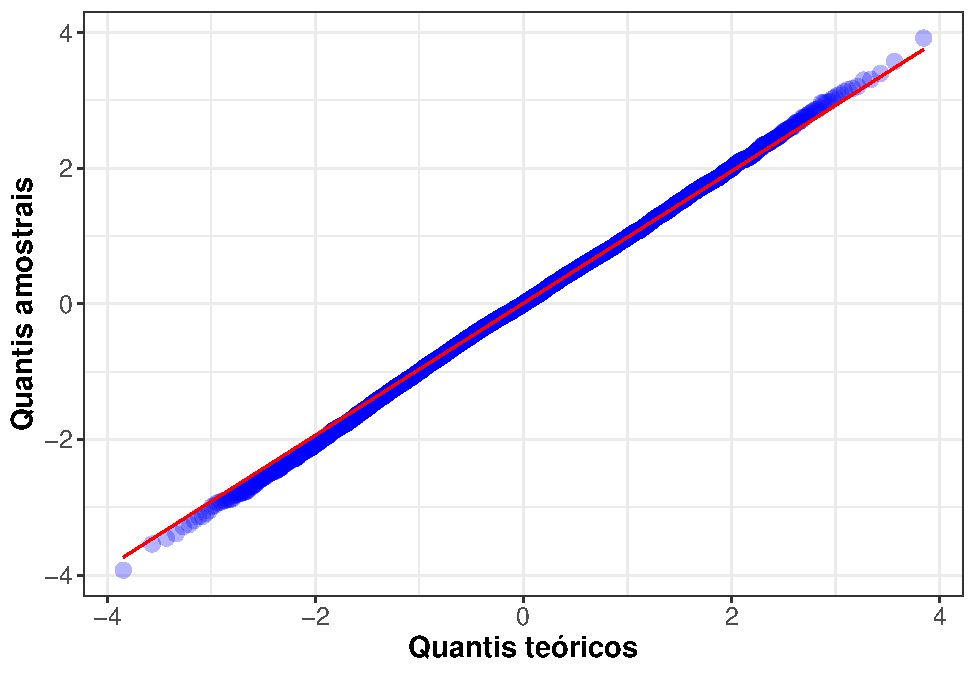
\includegraphics[width=1\linewidth]{article_files/figure-latex/qqplot-1} 

}

\caption{Gráfico quantil-quantil}\label{fig:qqplot}
\end{figure}

\hypertarget{anuxe1lise-e-interpretauxe7uxe3o-das-estimativas-dos-paruxe2metros}{%
\subsection{Análise e interpretação das estimativas dos parâmetros}\label{anuxe1lise-e-interpretauxe7uxe3o-das-estimativas-dos-paruxe2metros}}

A Tabela \ref{tab:coefs} apresenta as estimativas dos parâmetros do modelo para cada covariável utilizada. Através da estatística \(z\) de Wald, definida pela Equação \eqref{eq:wald}, onde \(\hat{\beta}_j\) é a estimativa de um particular parâmetro \(\beta_j\) do modelo e \(ep(\hat{\beta}_j)\) é o seu erro padrão, é possível obter a significância estatística de cada estimativa. Calculadas as estatísticas \(z\) de Wald, através da distribuição normal padrão a um determinado nível de significância obtemos os respectivos valores críticos e verificamos se estes rejeitam ou não a hipótese nula do teste \(z\) de Wald (\(H_0:\hat{\beta}_j=0\)) \cite{Favero2017}. Em outras palavras, o p-valor do teste \(z\) de Wald indica a probabilidade de \(\beta\) ser tão ou mais extremo que \(|z_{\hat{\beta}_j}|\).

\begin{equation}
z_{\hat{\beta}_j}=\dfrac{\hat{\beta}_j}{ep(\hat{\beta}_j)}\label{eq:wald}
\end{equation}

Através da Tabela \ref{tab:coefs} observa-se que todas as estimativas apresentaram significância ao nível de 5\%, não sendo necessária qualquer intervenção adicional no modelo final obtido a partir do algoritmo \textit{stepwise}.

\begin{table}

\caption{\label{tab:coefs}Estimativas dos parâmetros do modelo}
\centering
\fontsize{9}{11}\selectfont
\begin{tabular}[t]{lrrrr}
\toprule
Covariável & Estimativa & Erro padrão & Wald & P-valor\\
\midrule
Intercepto & 1.5513 & 0.1316 & 11.7902 & 0.0000\\
X2 & 0.3693 & 0.0387 & 9.5437 & 0.0000\\
X4 & -0.3558 & 0.0444 & -8.0085 & 0.0000\\
X5 & -0.2567 & 0.0487 & -5.2749 & 0.0000\\
X6 & -0.8296 & 0.1052 & -7.8829 & 0.0000\\
\addlinespace
X9 & 0.4532 & 0.1006 & 4.5028 & 0.0000\\
X11 & -0.3950 & 0.0697 & -5.6703 & 0.0000\\
X13 & -2.6981 & 0.1237 & -21.8040 & 0.0000\\
X14 & -2.2880 & 0.1246 & -18.3608 & 0.0000\\
X20 & 0.1598 & 0.0628 & 2.5453 & 0.0109\\
\addlinespace
X22 & -0.1925 & 0.0629 & -3.0595 & 0.0022\\
X27 & -0.1717 & 0.0748 & -2.2949 & 0.0217\\
X29 & -0.4516 & 0.0321 & -14.0894 & 0.0000\\
X30 & 0.4201 & 0.0457 & 9.1935 & 0.0000\\
X31 & -1.6460 & 0.0863 & -19.0675 & 0.0000\\
\bottomrule
\end{tabular}
\end{table}

Através da Equação \eqref{eq:odds}, obtida a partir da Equação \eqref{eq:logito}, é possível modelar a chance de ocorrência do evento de interesse para uma particular observação e, em consequência, avaliar o quanto a chance de ocorrência do evento de interesse se altera em média, em função de uma particular estimativa. Adicionalmente podemos dizer que o aumento de \(k\) unidades em uma particular covariável, mantidas as demais condições constantes, multiplica a chance de ocorrência do evento de interesse por \(e^{k\hat{\beta}_j}\), onde \(\hat{\beta}_j\) representa a estimativa do parâmetro desta particular covariável \cite{Favero2017}.

\begin{equation}
\dfrac{\pi_i}{1-\pi_i}= e^{\beta_0 + \beta_1 X_{i1} + ... +  \beta_p X_{ip}}\label{eq:odds}
\end{equation}

As Tabelas \ref{tab:odds} e \ref{tab:oddsmetricas} representam as estimativas dos parâmetros do modelo e estão ordenadas decrescentemente em função da variação absoluta da chance de ocorrência de \textit{churn}. Suas interpretações podem ser realizadas da seguinte forma, começando pela Tabela \ref{tab:odds}: a chance de \textit{churn} fica multiplicada por \(e^{-1,6460}=0,1928\) para 1 unidade a mais na covariável X31, mantidas as demais condições constantes. Em outras palavras, o acréscimo de 1 unidade na covariável X31 impacta na redução da chance de \textit{churn} em 81\%, fixadas as demais covariáveis. Como as covariáveis quantitativas foram padronizadas com média 0 e desvio padrão 1, é importante ressaltar que 1 unidade na covariável X31 não representa 1 dia de atividade, assim sendo, neste estudo a melhor forma de interpretar as estimativas dos parâmetros das covariáveis quantitativas é assimilando que estimativas menores que zero reduzem em média a chance de \textit{churn}, mediante ao aumento do valor de suas respectivas covariáveis, ao passo que a estimativa maior que zero aumenta em média a chance de \textit{churn}, à medida que o valor de sua respectiva covariável também aumenta, fixadas as demais covariáveis. Quanto às covariáveis qualitativas, também representadas na Tabela \ref{tab:odds}, podemos interpretá-las conforme o exemplo: a chance de \textit{churn} para os vendedores que estão no estágio I (X13) é 93\% menor com relação aos vendedores que não estão no mesmo estágio, mantidas as demais condições constantes. Por fim, com relação às covariáveis de desempenho (Tabela \ref{tab:oddsmetricas}), dadas as suas suas características representadas na Tabela \ref{tab:metricas}, suas interpretações podem ser realizadas de acordo com o exemplo: a chance de \textit{churn} de um vendedor que melhorou o seu desempenho nos subperíodos avaliados com relação ao faturamento (\(X6>0,5\)), é em média mais de 34\% menor, fixadas as demais covariáveis. Em contrapartida, a chance de \textit{churn} de um vendedor que piorou o seu desempenho nos subperídos avaliados com relação ao faturamento (\(X6<0,5\)), é também menor em média, entretanto, em um valor percentual inferior a 34.

Nesta etapa foi constatado que o aumento do número de dias em atividade no perído (X31), estar tanto no estágio I (X13) como no estágio R (X14) e a melhora do desempenho quanto ao faturamento (X6), são os fatores que mais impactam a redução da chance de \textit{churn}.

\begin{table}

\caption{\label{tab:odds}Chances de ocorrência de churn para covariáveis quantitativas e qualitativas}
\centering
\fontsize{9}{11}\selectfont
\begin{tabular}[t]{lrrr}
\toprule
Covariável & Estimativa & Chance & Variação (\%)\\
\midrule
X13 & -2.6981 & 0.0673 & -93\\
X14 & -2.2880 & 0.1015 & -90\\
X31 & -1.6460 & 0.1928 & -81\\
X30 & 0.4201 & 1.5221 & 52\\
X29 & -0.4516 & 0.6366 & -36\\
\addlinespace
X11 & -0.3950 & 0.6737 & -33\\
X22 & -0.1925 & 0.8249 & -18\\
X20 & 0.1598 & 1.1733 & 17\\
X27 & -0.1717 & 0.8422 & -16\\
\bottomrule
\end{tabular}
\end{table}

\begin{table}

\caption{\label{tab:oddsmetricas}Chances de ocorrência de churn para covariáveis de desempenho}
\centering
\fontsize{9}{11}\selectfont
\begin{tabular}[t]{lrrr}
\toprule
Covariável & Estimativa & Chance (0,5) & Variação (\%)\\
\midrule
X6 & -0.8296 & 0.6605 & -34\\
X9 & 0.4532 & 1.2543 & 25\\
X2 & 0.3693 & 1.2028 & 20\\
X4 & -0.3558 & 0.8370 & -16\\
X5 & -0.2567 & 0.8795 & -12\\
\bottomrule
\end{tabular}
\end{table}

\hypertarget{avaliauxe7uxe3o-do-poder-preditivo-do-modelo}{%
\subsection{Avaliação do poder preditivo do modelo}\label{avaliauxe7uxe3o-do-poder-preditivo-do-modelo}}

Para possibilitar a avaliação do poder preditivo do modelo na amostra de validação, é necessário antes definir o valor de \textit{cutoff}, ou seja, um ponto de corte de modo que as observações com probabilidade de ocorrência de \textit{churn} superior ao \textit{cutoff} sejam classificadas como \textit{churn} (\(Y=1\)) e, caso contrário, classificadas como não \textit{churn} (\(Y=0\)). A escolha do \textit{cutoff} foi realizada através da análise das curvas de sensibilidade e especificidade em função dos valores de \textit{cutoff}, e da curva ROC (\textit{Receiver Operating Characteristic}), gráfico que apresenta a variação da sensibilidade em função de (1 - especificidade), que mostra o comportamento do \textit{trade off} entre a sensibilidade e a especificidade em função da alteração do \textit{cutoff} \cite{Favero2017}. Atrávés do cálculo da área sob a curva ROC (AUC - \textit{Area Under the Curve}) é possível avaliar a eficiênca global do modelo, sendo \(AUC=1\) o melhor valor possível. O modelo em estudo apresentou \(AUC = 0,8894\), o que indica uma boa eficiência global. Analisadas as curvas de sensibilidade e especificidade (Figura \ref{fig:senscurve}) e a curva ROC (Figura \ref{fig:roc}), e considerando os requisitos do negócio, optou-se por um valor de \textit{cutoff} que garantisse o equilíbrio entre sensibilidade e especificidade. Portanto, para continuidade do estudo foram consideradas como \textit{churn} (Y=1) as observações com probabilidade de ocorrência de \textit{churn} superior a 0,55.

\begin{figure}

{\centering 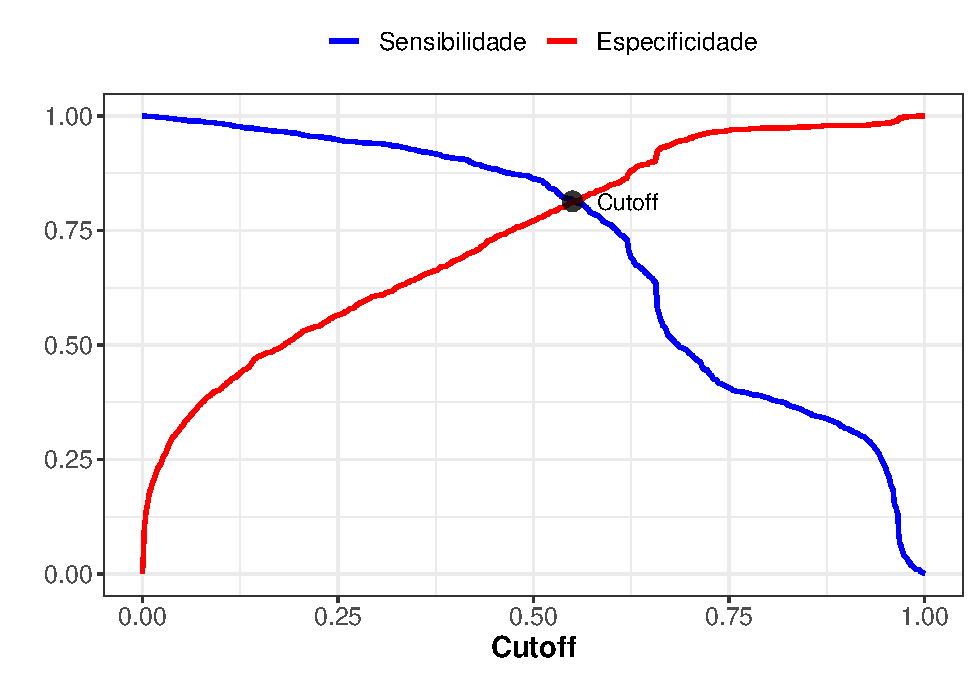
\includegraphics[width=1\linewidth]{article_files/figure-latex/senscurve-1} 

}

\caption{Curvas de sensibilidade e especificidade}\label{fig:senscurve}
\end{figure}

\begin{figure}

{\centering 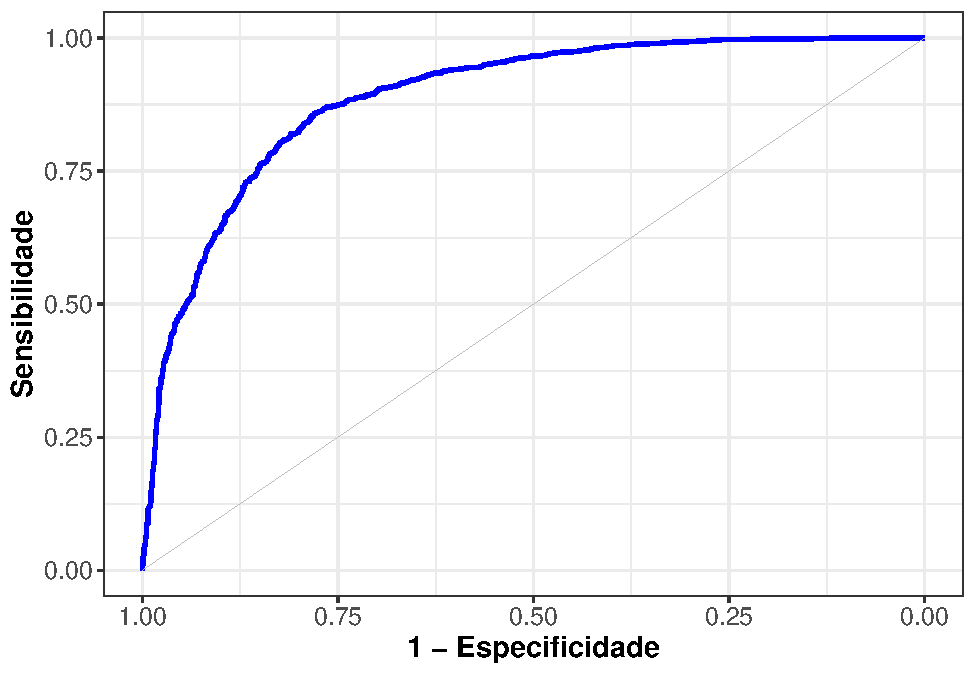
\includegraphics[width=1\linewidth]{article_files/figure-latex/roc-1} 

}

\caption{Curva ROC}\label{fig:roc}
\end{figure}

Definido o valor de \textit{cutoff}, através do cruzamento dos valores preditos pelo modelo e os valores observados, foi construída a matriz de confusão (Tabela \ref{tab:cmatrix}), que apresenta em sua diagonal principal o número de classificações corretas e, na diagonal secundária, o número de classificações incorretas. A partir da matriz de confusão foram calculadas as seguintes métricas de avaliação: sensibilidade (taxa de classificação correta entre as observações com a ocorrência de \textit{churn}), especificidade (taxa de classificação correta entre as observações sem a ocorrência de \textit{churn}) e acurácia (taxa global de classificações corretas), representadas pelas equações \eqref{eq:sensitivity}, \eqref{eq:specificity} e \eqref{eq:accuracy}, respectivamente.

\begin{table}

\caption{\label{tab:cmatrix}Matriz de confusão}
\centering
\fontsize{9}{11}\selectfont
\begin{tabular}[t]{lll}
\toprule
\multicolumn{1}{c}{} & \multicolumn{2}{c}{Observado} \\
\cmidrule(l{3pt}r{3pt}){2-3}
Predito & 0 & 1\\
\midrule
0 & Verdadeiro negativo (VN) & Falso negativo (FN)\\
1 & Falso positivo (FP) & Verdadeiro positivo (VP)\\
\bottomrule
\end{tabular}
\end{table}

\begin{equation}
S = \dfrac{VP}{VP+FN}\label{eq:sensitivity}
\end{equation}

\begin{equation}
E = \dfrac{VN}{VN+FP}\label{eq:specificity}
\end{equation}

\begin{equation}
A = \dfrac{VN+VP}{VN+VP+FN+FP}\label{eq:accuracy}
\end{equation}

Com a sensibilidade de 0,8164, especificidade de 0,8111 e acurácia de 0,8136 (com invervalo de confiança de 0,7986 a 0,8279), o poder preditivo do modelo foi considerado adequado para o negócio.

\hypertarget{conclusuxf5es}{%
\section{Conclusões}\label{conclusuxf5es}}

Através deste trabalho pretendeu-se construir um modelo para classificação de \textit{churn} interpretável e com poder preditivo adequado para o negócio. Entre as diversas técnicas disponíveis, a regressão logística foi escolhida por ser altamente confiável, por possibilitar a interpretação direta das estimativas dos parâmetros e por oferecer uma resposta na escala de probabilidade, permitindo aos decisores não só identificar os vendedores propensos a abandonar o relacionamento com a empresa, mas também ordená-los em função da probabilidade da ocorrência do \textit{churn}.

Por meio dos resultados apresentados, pôde-se constatar que o modelo proposto é capaz de atender a necessidade do negócio, uma vez que além do bom poder preditivo apresentado, oferece insights para ações de marketing personalizadas e otimizadas com foco na retenção dos vendedores propensos dar \textit{churn}.

Por fim, a abordagem utilizada na definição da variável resposta e na criação de métricas para avaliação de desempenho demonstrou-se eficaz no processo de modelagem, portanto, espera-se que este trabalho seja capaz de apoiar estudos futuros em condições semelhantes.

\hypertarget{agradecimentos}{%
\section{Agradecimentos}\label{agradecimentos}}

Ao Olist por prover todas as condições necessárias para o desenvolvimento do trabalho. Ao corpo docente da Especialização em \textit{Data Science} e \textit{Big Data} da Universidade Federal do Paraná - UFPR, pela qualidade do ensino oferecido, em especial ao Prof.~Walmes Zeviani pela orientação, inspiração e disponibilidade, inclusive nos finais de semana, e ao Prof.~Cesar Taconeli, que através das suas excelentes aulas me inspirou o interesse por Modelos Lineares Generalizados. Ao Prof.~Marcos Santos do Instituto Militar de Engenharia - IME, pelo suporte e incentivo à pesquisa.

\bibliographystyle{unsrt}
\bibliography{referencias}

\end{document}
